\chapter{Regression}
Regression is a very important topic in statistics that is applied extremely
frequently. There are many different kinds of regression, but in STATS 331 we will
mostly focus on linear regression. This gives us a nice familiar example
example to demonstrate how Bayesian statistics works and how it is different
from classical or frequentist statistics. Here we will study an example of a
simple linear regression problem taken from STATS 20X.

\section{A Simple Linear Regression Problem}
Data were collected from a sample of 30 drivers. The age of the driver and the 
maximum distance at which they could read a newly designed road sign were 
recorded. It is of interest to build a simple model that can be used to predict the 
maximum distance at which the sign is legible, using the age of the driver.
Figure~\ref{fig:road} shows the data.
\begin{figure}
\begin{center}
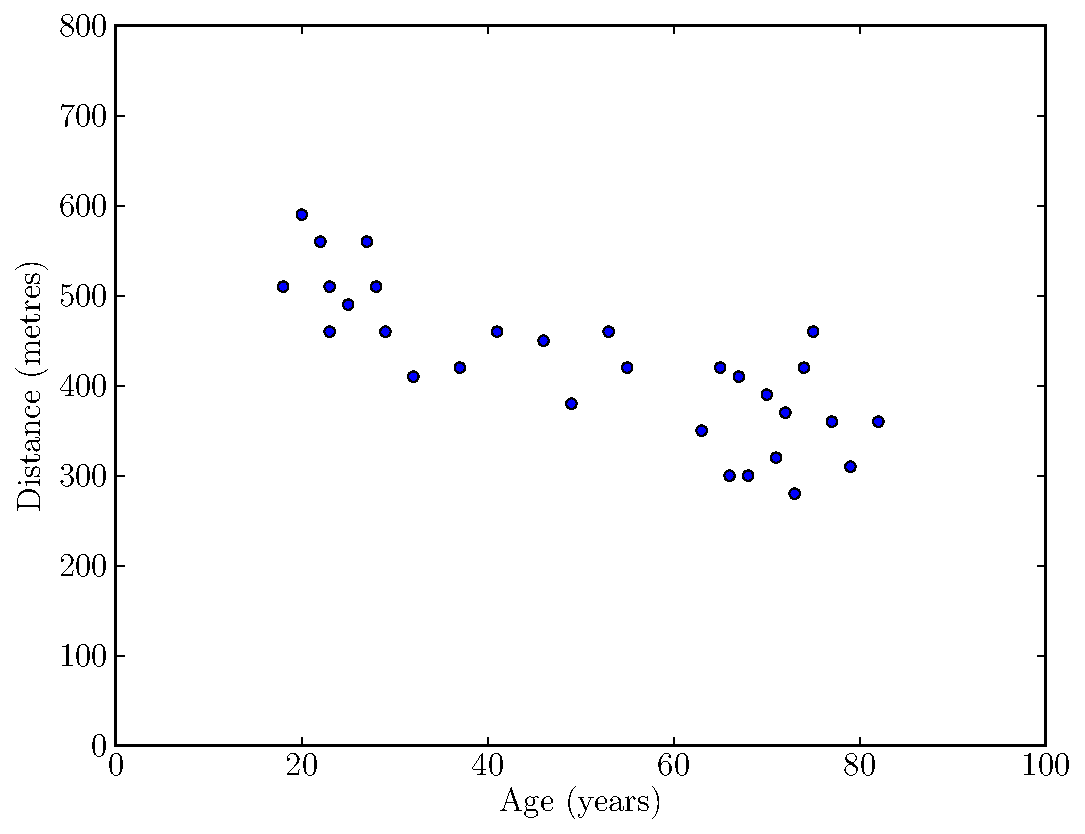
\includegraphics[scale=0.5]{Figures/road.pdf}
\caption{\it The maximum distance at which a person can read a road sign vs. the age of
the person. There are $N=30$ data points. You can clearly see that older people
have, on average, worse eyesight. Simple linear regression can be thought of as
``fitting a straight line'' to the data.
\label{fig:road}}
\end{center}
\end{figure}
The purpose of simple linear regression is to find a straight line that goes
throught the data points. The slope and intercept of the straight line are then
helpful for understanding the relationship between the variables. Also, the straight line can be used
to predict future data, such as the maximum distance at which a 90-year-old person
could read the sign. The most common method used to obtain the straight
line is to find the line (i.e. the slope and intercept values) which fits best
by the criterion of ``least squares''.

\section{Interpretation as a Bayesian Question}
From what you now know about Bayesian statistics, you might be able to come up
with some reasons why the standard least squares
solution is unsatisfactory. One glaring issue is that the data are hardly ever
going to be good enough to tell us with certainty that a particular slope and intercept
are correct (the exception would be if three or more points lie perfectly on a straight
line, with no scatter).
In principle, we will almost always have uncertainty about the slope and
the intercept. From a Bayesian perspective, our goal is not to find a point
estimate for the slope and the intercept. Instead we should calculate the
{\it posterior distribution for the slope and the intercept, given the data}.
The posterior distribution will tell us exactly how much uncertainty we have.
If we do want summaries for convenience, we can use the posterior distribution
to create the summaries, as discussed in Chapter~\ref{chapter:summaries}.

The equation for a straight line is usually written as $y = mx + b$ where $m$
is the gradient/slope and $b$ is the intercept. However,
for consistency with later, more complex regression models, we will write the
equation as:
\begin{eqnarray}
y = \beta_0 + \beta_1 x.
\end{eqnarray}
Here, $\beta_0$ is the $y$-intercept and $\beta_1$ is the slope. Our goal is
to calculate the posterior distribution for $\beta_0$ and $\beta_1$ given the
data.

\section{Analytical Solution With Known Variance}
Bayes' rule (parameter estimation version) tells us how to calculate the
posterior distribution:
\begin{eqnarray}
p(\theta|x) \propto p(\theta)p(x|\theta)
\end{eqnarray}
This is the generic form for parameters $\theta$ and data
$x$. In our particular case, the
unknown parameters are $\beta_0$ and $\beta_1$, and the data are the
$y$ values of the data points. The data also consist of a number $N$ of points
and the $x$-values,
but we shall assume that these on their own provide no information about the
slope and intercept (it would be a bit strange if they did). So the $x$-values
and the number of points $N$ act like prior information that lurks ``in the
background'' of this entire analysis. The $y$-values are our data in the sense
that we will obtain our likelihood by writing down a probability distribution
for the $y$-values given the parameters.

Therefore, Bayes' rule {\it for this problem} (i.e. with the actual names
of our parameters and data, rather than generic names) reads:
\begin{eqnarray}
p(\beta_0, \beta_1 | y_1, y_2, ..., y_N) \propto
p(\beta_0, \beta_1)p(y_1, y_2, ..., y_N | \beta_0, \beta_1)
\end{eqnarray}

We can now say some things about Bayesian linear regression by working
analytically. For starters, 
let's assume uniform priors for both $\beta_0$ and $\beta_1$, and that the
prior for these two parameters are independent. The probability density for
a uniform prior distribution can be written simply as:
\begin{eqnarray}
p(\beta_0, \beta_1) \propto 1.
\end{eqnarray}
Note that we have written proportional instead of equals. If we decided to
place the limits at -500 and 500 (say) then the actual value of the density
would be $10^{-6}$. But this is just a number and in the end, when we normalise
the posterior distribution, it won't matter. We can even imagine making our
prior ``infinitely wide'', which is called an improper prior. In many cases
simply writing $p(\beta_0, \beta_1) \propto 1$ will not cause any problems. We
are assuming the prior probability density is uniform over a very wide range
which we will not specify.

Now, on to the likelihood. There are $N$ data points and so there are $N$
$y$-values in the dataset, called $\{y_1, y_2, ..., y_N\}$. We can obtain the
likelihood by writing down a probability distribution for the data given the
parameters, sometimes called a ``sampling distribution''. This describes our
beliefs about the connection between the data and the parameters, without which
it would be impossible to learn anything from data.
If we
knew the true values of $\beta_0$ and $\beta_1$, then we would predict the
$y$-values to be scattered around the straight line. Specifically we
will assume that each point departs from the straight line by an amount
$\epsilon_i$ which has a $\mathcal{N}(0, \sigma^2)$ probability distribution.
For now, we will assume $\sigma$, the standard deviation of the scatter, is known.
In ``$\sim$'' notation, this can be written as:
\begin{eqnarray}
y_i \sim \mathcal{N}(\beta_0 + \beta_1 x_i, \sigma^2).
\end{eqnarray}
It is implied that all of the data values are independent (given the
parameters). Therefore the likelihood can be written as a product of $N$
normal densities, one for each data point:
\begin{eqnarray}
p(\{y_1, y_2, ..., y_N\}|\beta_0, \beta_1) &=& \prod_{i=1}^N \frac{1}{\sigma\sqrt{2\pi}}
\exp\left[-\frac{1}{2\sigma^2}\left(y_i - (\beta_0 + \beta_1 x_i)\right)^2\right].
\end{eqnarray}
Remember, when we combine the likelihood with the prior using Bayes' rule,
we can usually ignore any constant factors which do not depend on
the parameters. This allows us to ignore the first part of the product, outside
the exponential (since we are assuming $\sigma$ is known).
\begin{eqnarray}
p(\beta_0, \beta_1 | y_1, y_2, ..., y_N) &\propto& p(\beta_0, \beta_1)
p(y_1, y_2, ..., y_N|\beta_0, \beta_1)\\
&\propto& 1 \times \prod_{i=1}^N \exp\left[-\frac{1}{2\sigma^2}\left(y_i - (\beta_0 + \beta_1 x_i)\right)^2\right]\\
&\propto& \exp\left[-\frac{1}{2\sigma^2}\sum_{i=1}^N\left(y_i - (\beta_0 + \beta_1 x_i)\right)^2\right].
\label{eq:leastsquares}
\end{eqnarray}
We have just found the expression for the posterior distribution for $\beta_0$
and $\beta_1$. This is a distribution for two parameters (i.e. it is bivariate).
It is not easy to interpret this equation just by
looking at it, but we could use it to work out the value of the posterior
probability density for any possible values of $\beta_0$ and $\beta_1$

There are a few things you may notice about the posterior distribution in
Equation~\ref{eq:leastsquares}. Firstly, the way it depends on the parameters
is an exponential of something involving $\beta_0$
and $\beta_1$ in linear and second-order ways (if you were to expand the square,
you would get terms like $\beta_0\beta_1$ and $\beta_0^2$). Mathematicians would
call the expression inside the exponential a {\it quadratic form}. When a
probability density can be written as the exponential of a quadratic form, it
is a normal density. Therefore, the posterior distribution for $\beta_0$ and
$\beta_1$ is a (bivariate) normal distribution.

We can obtain some more insight about this problem by inspecting the
sum term inside the exponential in the posterior distribution
(Equation~\ref{eq:leastsquares}). The sum is over all the data points, and
what is being summed is the difference between the data value $y_i$ and the
straight line prediction $\beta_0 + \beta_1 x_i$, all squared.
The sum term is just the sum of squared
residuals that is minimised when solving this problem by ``least squares''.
In classical least squares linear regression, $\beta_0$ and $\beta_1$ are
estimated by minimising this sum of squared residuals. Because of the exp and
the minus sign, the posterior distribution is telling us that the choice of
$\beta_0$ and $\beta_1$ that minimises the sum of squared residuals, maximises
the posterior probability density. Other values of the parameters that
don't quite minimise the sum of squared residuals are somewhat plausible, and
the form of the posterior density tells us exactly how much less plausible they
are. The take home message is summarised below.

\begin{framed}
{\bf Doing a linear regression by least squares is equivalent to having a
uniform prior and a normal likelihood, and finding the posterior mode.
If you think this is appropriate in a particular application, and you are happy
with just a point estimate, then classical
least squares fitting will be fine. Otherwise, you'd better do a Bayesian analysis.}
\end{framed}

While classical regression results may come with ``standard errors'', these are
not the same as a posterior distribution. A posterior distribution describes the
uncertainty about the parameters given the specific data set you actually have.
Standard errors describe how different your point estimate would be if your data
set was different.

\section{Solution With JAGS}
The above analytical results made the unrealistic assumption that the standard
deviation $\sigma$, of the scatter, was known. In practice, $\sigma$ usually needs to be
estimated from the data as well. Therefore, in the Bayesian framework, we should
include it as an extra unknown parameter. Now we have three unknown parameters instead
of two. Our parameters are now $\beta_0$, $\beta_1$, and $\sigma$.
One major advantage of MCMC is that we can increase the number of unknown parameters
without having to worry about the fact that the posterior distribution might
be hard to interpret or plot.

The data is the same as before, $\{y_1, y_2, ..., y_N\}$. The likelihood is
also the same as before:
\begin{eqnarray}
y_i \sim \mathcal{N}(\beta_0 + \beta_1 x_i, \sigma^2).
\end{eqnarray}

Our three parameters will need priors. JAGS requires proper priors (i.e. we
can't have a uniform prior over an infinite range), but we can still make our
priors very wide. Instead of using uniform distributions this time,
we will use normal distributions with a mean of 0 and a large standard deviation
of 1000.

For the standard deviation parameter $\sigma$, we know firstly that this cannot
be negative. We will use a ``log-uniform'' prior with generous lower and upper limits,
to express uncertainty about the order of magnitude of $\sigma$. This prior implies
things like $P(1 < \sigma < 10) = P(10 < \sigma < 100) = P(100 < \sigma < 1000)$,
which is sometimes a good description of a large amount of uncertainty about
a positive parameter. The easiest way to implement this in JAGS is to actually
use $\log(\sigma)$ as the parameter, with a uniform prior, and then define
$\sigma = \exp\left(\log(\sigma)\right)$. Notice that ``deterministic nodes''
(quantities that are defined in terms of other variables) in JAGS are defined
using ``{\tt <-}'' instead of ``{\tt \~{ }}''.

In JAGS, the model looks like this:
\begin{minted}[mathescape,
               numbersep=5pt,
               gobble=0,
               frame=single,
               framesep=2mm, fontsize=\small]{r}
model
{
  # Prior for all the parameters
  beta0 ~ dnorm(0, 1/1000^2)
  beta1 ~ dnorm(0, 1/1000^2)
  log_sigma ~ dunif(-10, 10)
  sigma <- exp(log_sigma)

  # Likelihood
  for(i in 1:N)
  {
    y[i] ~ dnorm(beta0 + beta1*x[i], 1/sigma^2)
  }
}
\end{minted}

The first part defines the priors for the parameters. For $\beta_0$ and $\beta_1$,
we have just chosen very broad priors that describe vague prior knowledge. Note
that the standard deviations of the priors are 1000, so we should be careful
to only apply this code in situtations where we don't expect the intercept or
slope to have an extreme value (either positive or negative).

For the standard deviation parameter $\sigma$, which describes how much we
expect the data points to be scattered around the straight line, we have assigned
a log-uniform prior. The limits of $-10$ and $10$ for {\tt log\_sigma} imply
limits of $4.5 \times 10^{-5}$ to 22,000 for {\tt sigma}, a generous range.
If we thought $\sigma$
might actually be outside this range, we should change the prior to something
else or risk getting strange answers.

The likelihood part of the code involves a {\tt for} loop, because our data
is more than just a single number. The code inside the loop is effectively
duplicated $N$ times (with $i=1$, then with $i=2$, etc), once for each data
point. Since the loop refers to a quantity {\tt N}, this must be specified in
the {\tt data} list if you are using my {\tt use\_jags.r} template code.

Another new feature of this JAGS model is the normal distribution, which is
called {\tt dnorm} in JAGS. Usually a normal distribution is written
$\mathcal{N}(\mu, \sigma^2)$ where $\mu$ is the mean and $\sigma$ is the standard
deviation (and $\sigma^2$ is the variance). Unfortunately, in JAGS there is a
quirk: the first argument to {\tt dnorm} is indeed the mean, but the second argument
must be one over the variance, or one over the standard deviation squared.

\section{Results for ``Road'' Data}
Our JAGS output will contain samples from the posterior distribution for
$\beta_0$, $\beta_1$ and $\sigma$. The first thing we should do is make
trace plots and check that everything converged properly. Then we can make
histograms of each parameter to visually inspect the (marginal) posterior
distribution for each parameter. We can also plot one parameter vs. another
to look at the {\it joint} posterior distribution for the parameters. R code
for all of these is given below.

\begin{minted}[mathescape,
               numbersep=5pt,
               gobble=0,
               frame=single,
               framesep=2mm, fontsize=\small]{r}
# Plot trace plots
plot(results$beta0, type='l', xlab='Iteration', ylab='beta0')
plot(results$beta1, type='l', xlab='Iteration', ylab='beta1')
plot(results$sigma, type='l', xlab='Iteration', ylab='sigma')

# Plot histograms
hist(results$beta0, breaks=20, xlab='beta0')
hist(results$beta1, breaks=20, xlab='beta1')
hist(results$sigma, breaks=20, xlab='sigma')

# Plot joint posterior distribution of beta0 and beta1
plot(results$beta0, results$beta1, cex=0.1, xlab='beta0', ylab='beta1')
\end{minted}

All of the plots for the road data are shown in Figure~\ref{fig:road_results}.
\begin{figure}[!ht]
\begin{center}
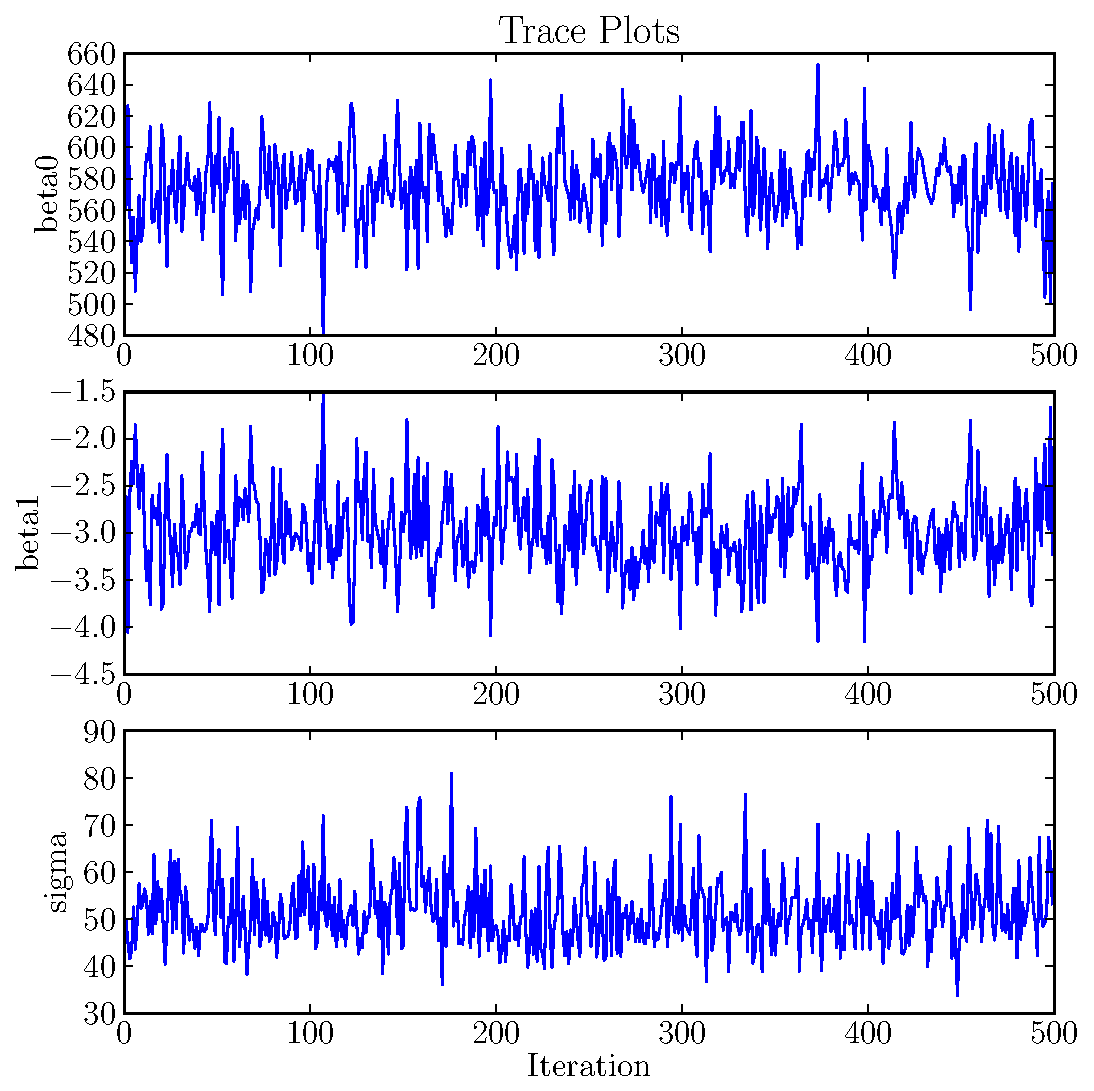
\includegraphics[scale=0.35]{Figures/road_trace.pdf}
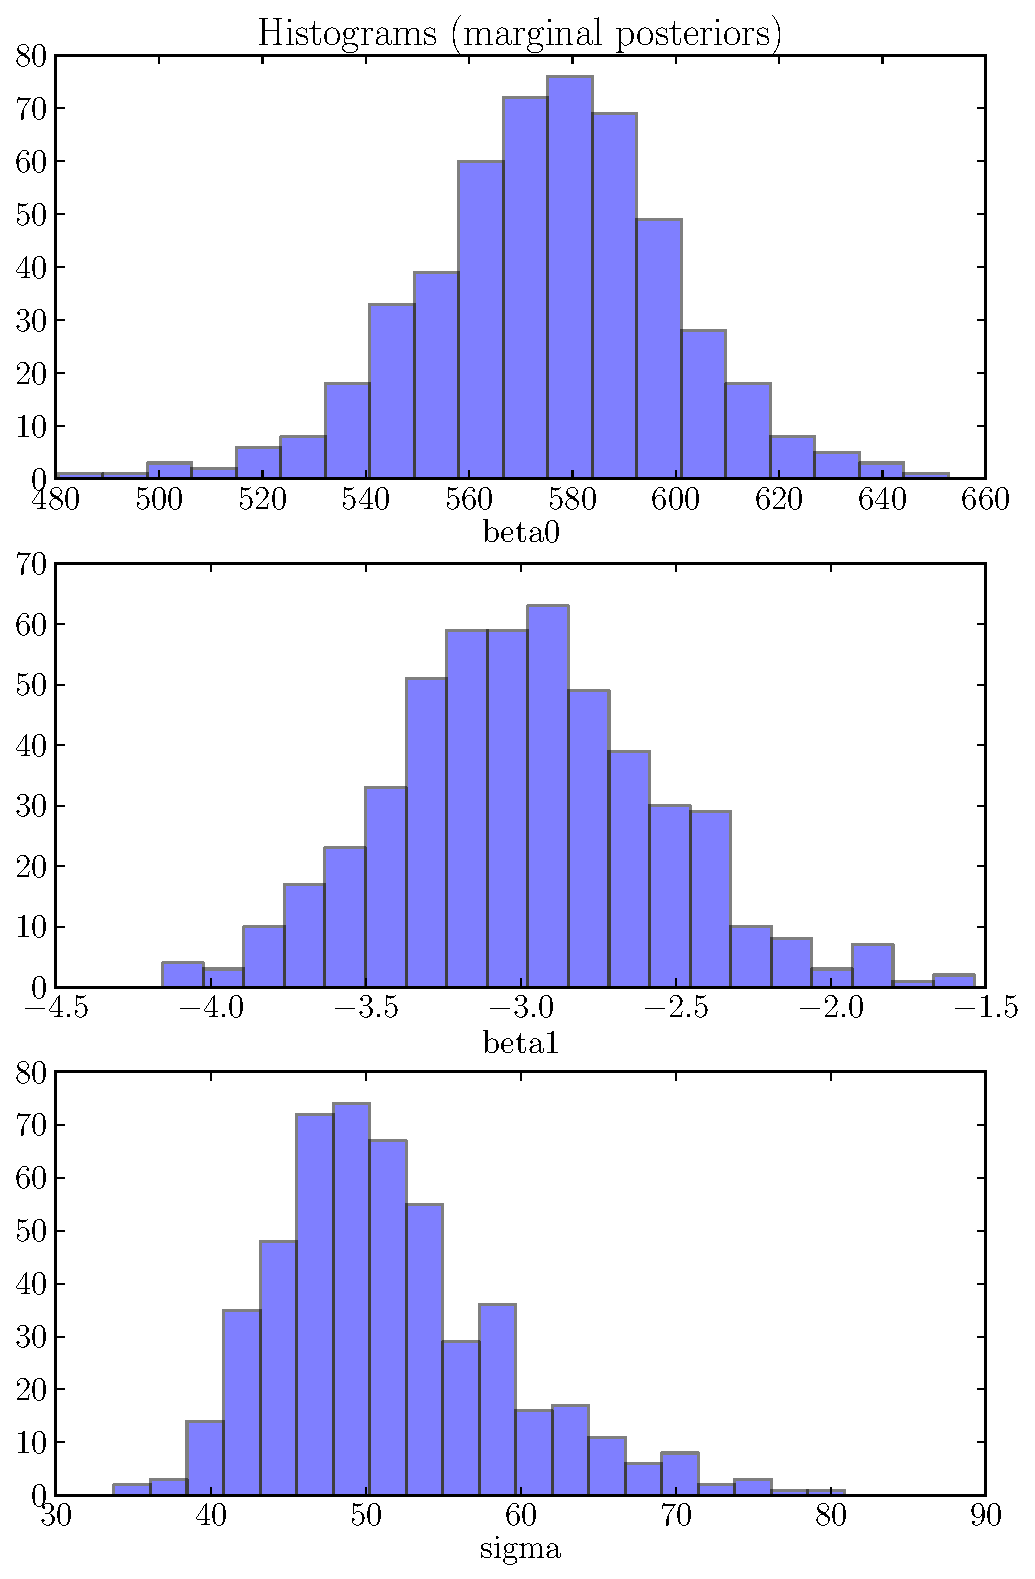
\includegraphics[scale=0.35]{Figures/road_hist.pdf}
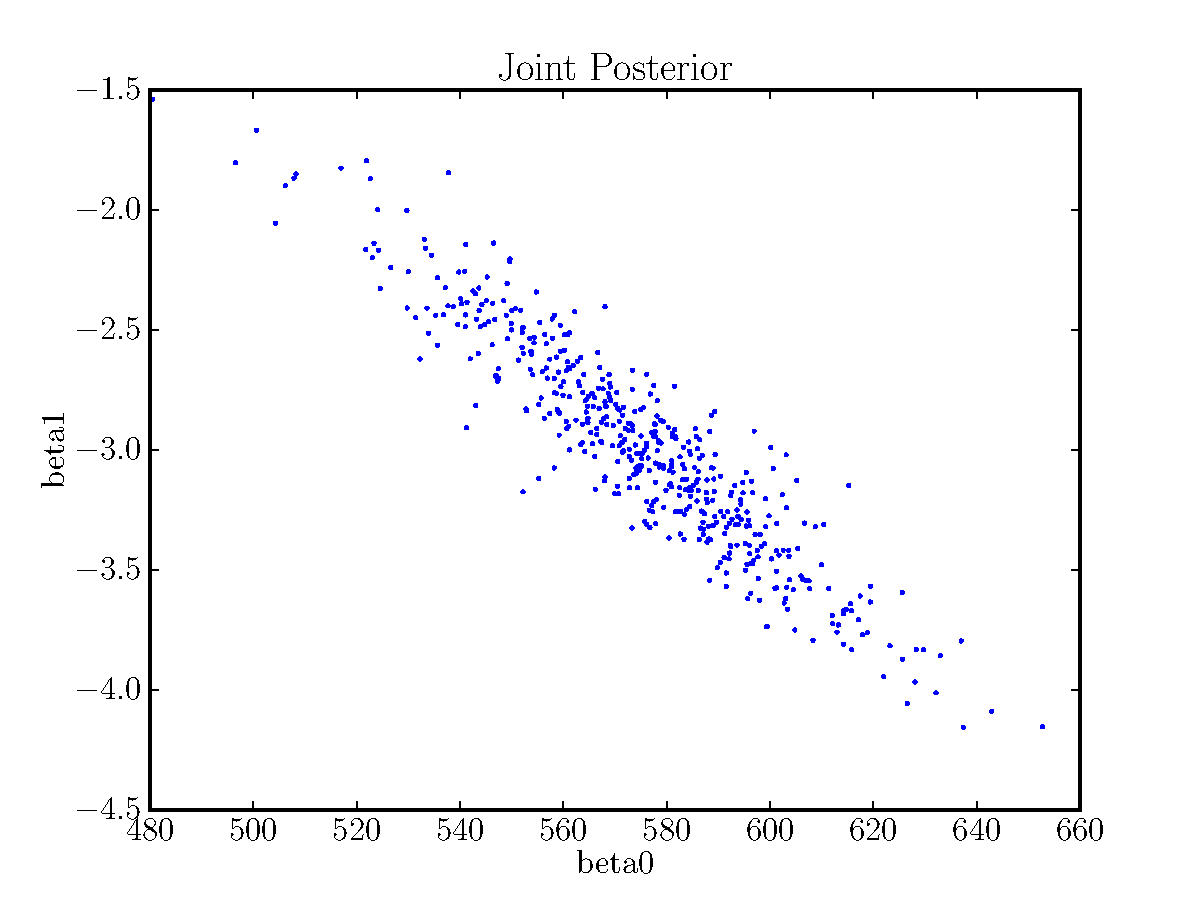
\includegraphics[scale=0.35]{Figures/road_joint.pdf}
\caption{\it Results (posterior samples) from the simple linear regression model
applied to the road data.
{\bf Top Left}: Trace plots showing the parameters moving around over time (as the
MCMC progressed). 
{\bf Top Right}: Histograms of the posterior samples, showing the marginal
posterior distributions for the parameters.
{\bf Bottom}: A plot of $\beta_1$ vs. $\beta_0$, showing samples from the joint
posterior for these two parameters. These parameters had independent priors, but
the posterior shows a correlation. All this means is that if $\beta_0$ is a
high value then $\beta_1$ must be low, and vice versa.
\label{fig:road_results}}
\end{center}
\end{figure}

With classical linear regression it is usually helpful to plot the best fitting
line through the data. In Bayesian linear regression our output is posterior
samples for what the parameters might be (and therefore what the line might be).
A common way of displaying the posterior is to plot many lines through the data,
with the lines produced using the posterior samples. Some R code for doing this
is given below. The plot produced looks like the one in
Figure~\ref{fig:road_lines}.

\begin{minted}[mathescape,
               numbersep=5pt,
               gobble=0,
               frame=single,
               framesep=2mm, fontsize=\small]{r}
# Plot the data
plot(data$x, data$y)

# Make some x-values for plotting lines
x = c(0, 100)
# Plot the first 30 lines from the posterior distribution
for(i in 1:30)
{
    lines(x, results$beta0[i] + results$beta1[i]*x)
}
\end{minted}


\begin{figure}[!ht]
\begin{center}
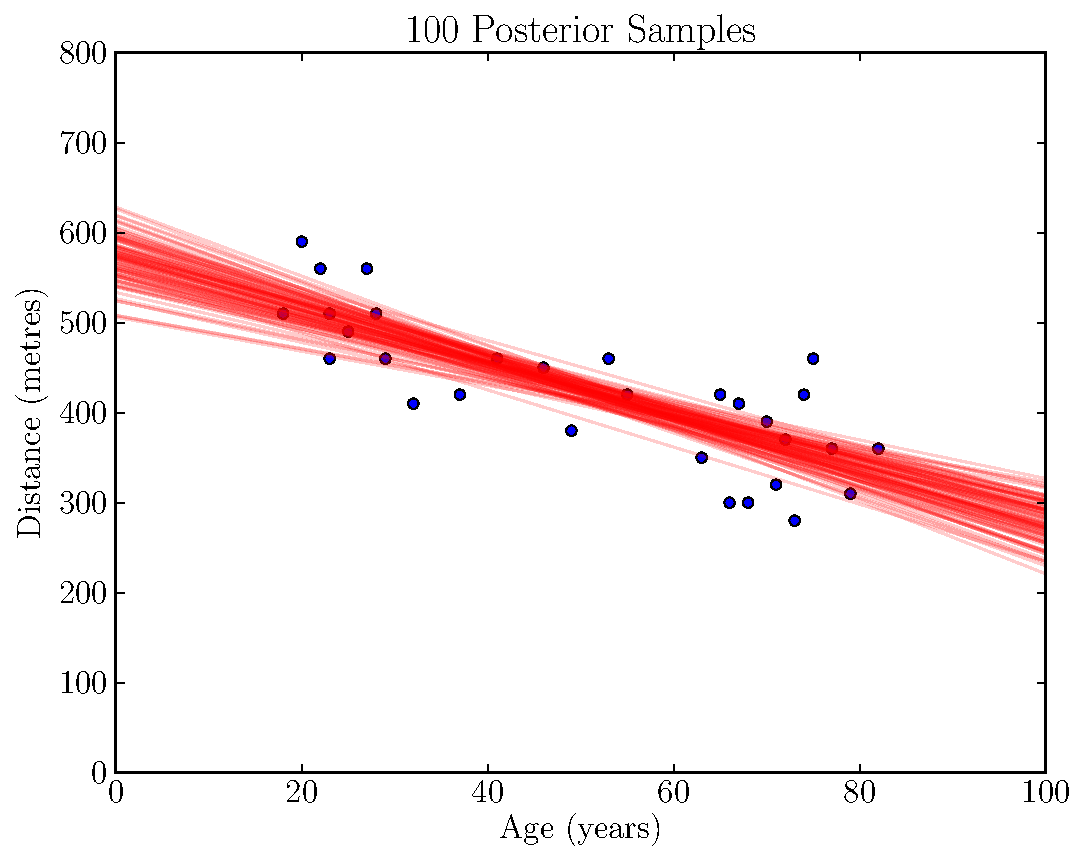
\includegraphics[scale=0.5]{Figures/road_lines.pdf}
\caption{\it The road data with credible regression lines (sampled from the
posterior distribution) overplotted.\label{fig:road_lines}}
\end{center}
\end{figure}

\section{Predicting New Data}
One of the most important uses of regression models is for prediction. Given
this data, what can we say about the value of the output variable $y$ at some
new value of the input variable, $x_{\rm new}$? It's unknown, but let's call it
$y_{\rm new}$. With our road example, we will try to predict the maximum reading
distance of a person who is $x_{\rm new}=90$ years old.
If we knew the parameters of the straight line (or had a good point estimate),
we could extend it out to $x=90$, and compute our predicted value:

\begin{eqnarray}
y_{\rm new} &=& \beta_0 + \beta_1 x_{\rm new}\\
&=& \beta_0 + \beta_1\times 90
\end{eqnarray}
but that's not quite in the Bayesian spirit. Firstly, we don't know the value
of the parameters, we only have the posterior distribution. Secondly, we would
like not just a point estimate for $y_{\rm new}$ but a whole probability distribution,
describing all of the uncertainty in the prediction. One simple improvement
would be to state that our uncertainty about $y_{\rm new}$ should be described
by a normal distribution around the straight line, with standard deviation $\sigma$.
This still isn't quite right though, because we'd need to know the true values
of the parameters to actually do it.

In general, Bayesian prediction works like so. With parameters
$\theta$ and data $x$, we can predict ``new data'' $x'$ by calculating the
``posterior predictive distribution'' which is just the probability distribution
for $x'$ given $x$:
\begin{eqnarray}
p(x' | x) &=& \int p(\theta, x' | x) \, d\theta\\
&=& \int p(\theta|x) p(x' | x, \theta)\, d\theta
\end{eqnarray}
We first saw this in Section~\ref{sec:prediction_bus_problem}.
The first term inside the integral is the posterior, and therefore the
whole integral is an expectation value, with respect to the posterior distribution.
The second term is
the probability distribution for $x'$ given the parameters, i.e. imagining that
we knew the parameters.

This equation is telling us to imagine that we know the
true parameter values, make a prediction (in terms of a probability distribution),
repeat this for all possible parameter values
and then average together all the probability distributions into one ``final''
distribution. In the averaging process we should give more weight
to the probability distributions that were based on plausible values of $\theta$.

Thankfully, actually doing this is much easier than it sounds, thanks to MCMC.
Remarkably, we can accomplish all this, and obtain our probability distribution
for $y_{\rm new}$, by adding just a single line to the JAGS model:
\begin{minted}[mathescape,
               numbersep=5pt,
               gobble=0,
               frame=single,
               framesep=2mm, fontsize=\small]{r}
y_new ~ dnorm(beta0 + beta1*90, 1/sigma^2)
\end{minted}
Of course, to look at the posterior samples for {\tt y\_new}, you'll need to
monitor it. The samples of {\tt y\_new}
will be drawn from the posterior predictive distribution for the new data.
Internally, JAGS will simulate a new value of {\tt y\_new} at every iteration,
from the specified distribution, and using its current estimates of the parameters.
Since the parameters are not fixed, but explore the posterior distribution, the
distribution of {\tt y\_new} values will take into account all of the uncertainty
we have about the parameter values.

As a general rule for predicting new data in JAGS, the extra line(s) you'll add to the JAGS
model will usually resemble the likelihood, but the variable will have a different name.
The results for the road data prediction are shown
in Figure~\ref{fig:road_prediction}.
\begin{figure}[!ht]
\begin{center}
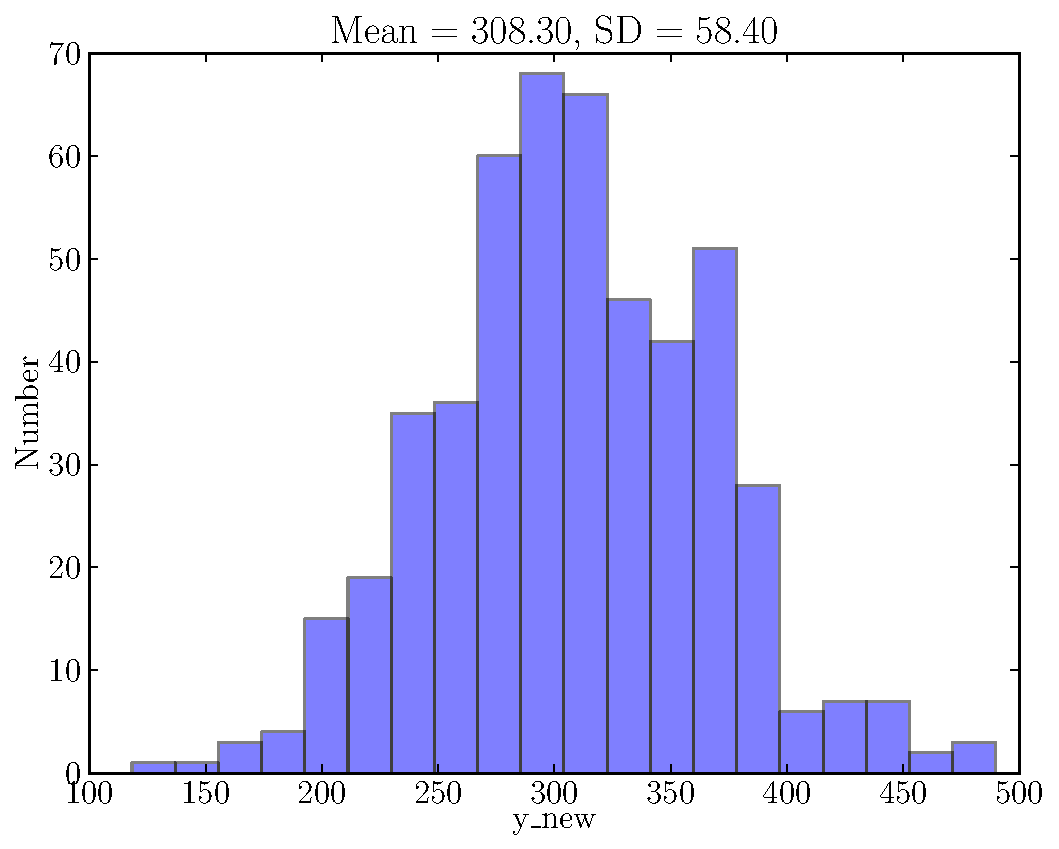
\includegraphics[scale=0.5]{Figures/road_prediction.pdf}
\caption{\it Samples from the posterior predictive distribution, answering the
question ``what do we know about $y$ at $x=90$?''. Summaries are shown in
the title. If we simply assumed the best fit line was true and applied a
point estimate of $\sigma$ to get our uncertainty, we would have obtained a
prediction of $306.07 \pm 49.76$.\label{fig:road_prediction}}
\end{center}
\end{figure}

\section{Simple Linear Regression With Outliers}
One complication that is common in linear regression (or other model-fitting)
problems is the existence of outliers. These are points that do not fit in with
the general trend assumed by the model. Many methods exist for deciding how to
``detect'' and ``remove''
outliers. From a Bayesian point of view, there is not a one-size-fits-all approach
to outliers. If you really believe in your model assumptions, an ``outlier''
might be your most important data point. If you aren't really sure of your
model assumptions and are just using a convenient default model, then your results
may be misleading.
In lectures and labs we will study an extension to the simple linear
regression model that allows for outliers by using a heavier-tailed sampling
distribution, the Student-$t$ distribution.

\section{Multiple Linear Regression and Logistic Regression}
We will study an example of multiple linear regression, and nonlinear regression
(involving an ``interaction term'') in lectures.
We will not study a logistic regression explicitly, but the special
lecture on predicting sports matches is very closely related to logistic
regression. The main difference between linear regression is that the output
variable can only be 0 or 1, so the likelihood will usually involve the
``Bernoulli'' distribution (a Binomial distribution with one trial).

